%Semantics of state charts
\section{\plcchart s}
\label{sec:statechartsem}

The language used for our project was purposely modelled after \emphasize{UML2 State Machine Diagram}\cite{UML2}. As discussed in section \ref{sec:overviewstatechart} UML2 is essentially standard state machine with extensions added on to describe behaviours in states. The motivation in using \emphasize{UML2 State Machine Diagram}\cite{UML2} as a basis for our state machine system consists of three primary details: First \emphasize{UML2 State Machine Diagram}\cite{UML2} is quite well known and popular, this improves the potential acceptance of our tool. Secondly \emphasize{UML2 State Machine Diagram}\cite{UML2} state machine syntax is more concrete than the other forms of state machines, giving a strong basis to construct our language around. Finally \emphasize{UML2 State Machine Diagram}\cite{UML2} has the concept of internal activity or internal execution necessary for modelling the behaviour of an actual useful program.

The model of \plcchart $\:$ is expressed mathematically as follows:

\begin{definition}
	\plcchart
	
\begin{itemize}
	\item \textbf{$Q$:} Set of modes.
	\item \textbf{$V$:} The state space $V = \langle V_0,V_1,V_2,..,V_n \rangle \: where \: V_{i}\in \lbrace \mathbb{Z}_{128}, \mathbb{Z}, \mathbb{B}, \mathbb{R} \rbrace$
	\item $\mathbf{v}_{init}$: vector of initial values $\mathbf{v}_{init}$: $\langle v_0,..,v_n \rangle \: where \: (v_i \in V_i)$
	\item \textbf{$G$:} Set of guard conditions. $V \rightarrow \mathbb{B}$
	\item \textbf{$A$:} Set of assignments. $V \times Q \rightarrow V$
	\item \textbf{$\tau$:} Set of transitions. $G \times Q \rightarrow Q$
	\item \textbf{$q_0$:} The initial starting mode.
\end{itemize}
\end{definition}

In each mode the system is in one or many different states. State spaces in our system are used for variable assignments and all variables are typed. Initial values in the system are given by a vector of elements that come from the state spaces $V$.  Guard conditions are mappings from states spaces to boolean values.

Assignments in our system take the form $V \times Q \rightarrow V$. Suppose we have variables $\langle 1,2 \rangle$ mode $5$ one possible assignment is then $( \langle 1,2 \rangle,5) \rightarrow ( \langle 2,0 \rangle )$. Assignments can be in the form of a constant or an equation.

%\begin{align}
%v_1 := v_0 \label{eqn:assign0} \\ 
%v_0 := v_1 \label{eqn:assign1}
%\end{align}

%\begin{align}
%(v_1,q_1) \rightarrow v_0 \label{eqn:assign0} \\ 
%(v_0,q_1) \rightarrow v_1 \label{eqn:assign1}
%\end{align}
%
%We would see that the result $v_1 = v_0$ it is important to note this since generally in \emphasize{Finite State Machines}\cite{booth}  it is understood that assignments happen concurrently in such a case equations \ref{eqn:assign0} and \ref{eqn:assign1} would produce a swap where $v'_1 = 'v_0$ and $v'_0 = 'v_1$ (where $'v$ denotes the value of $v$ before the assignments are made and $v'$ the value of $v$ after the assignment is completed). In normal state machines we read assignments such as in equations \ref{eqn:assign0} and \ref{eqn:assign1} as these assignments will take place upon entry of the state. For our semantics however, we read them in a sequential fashion for example: Upon entry of the mode, first equation \ref{eqn:assign0} is assigned, then \ref{eqn:assign1} right afterwards.
%
%\begin{figure}[htp]
%    \centering
%    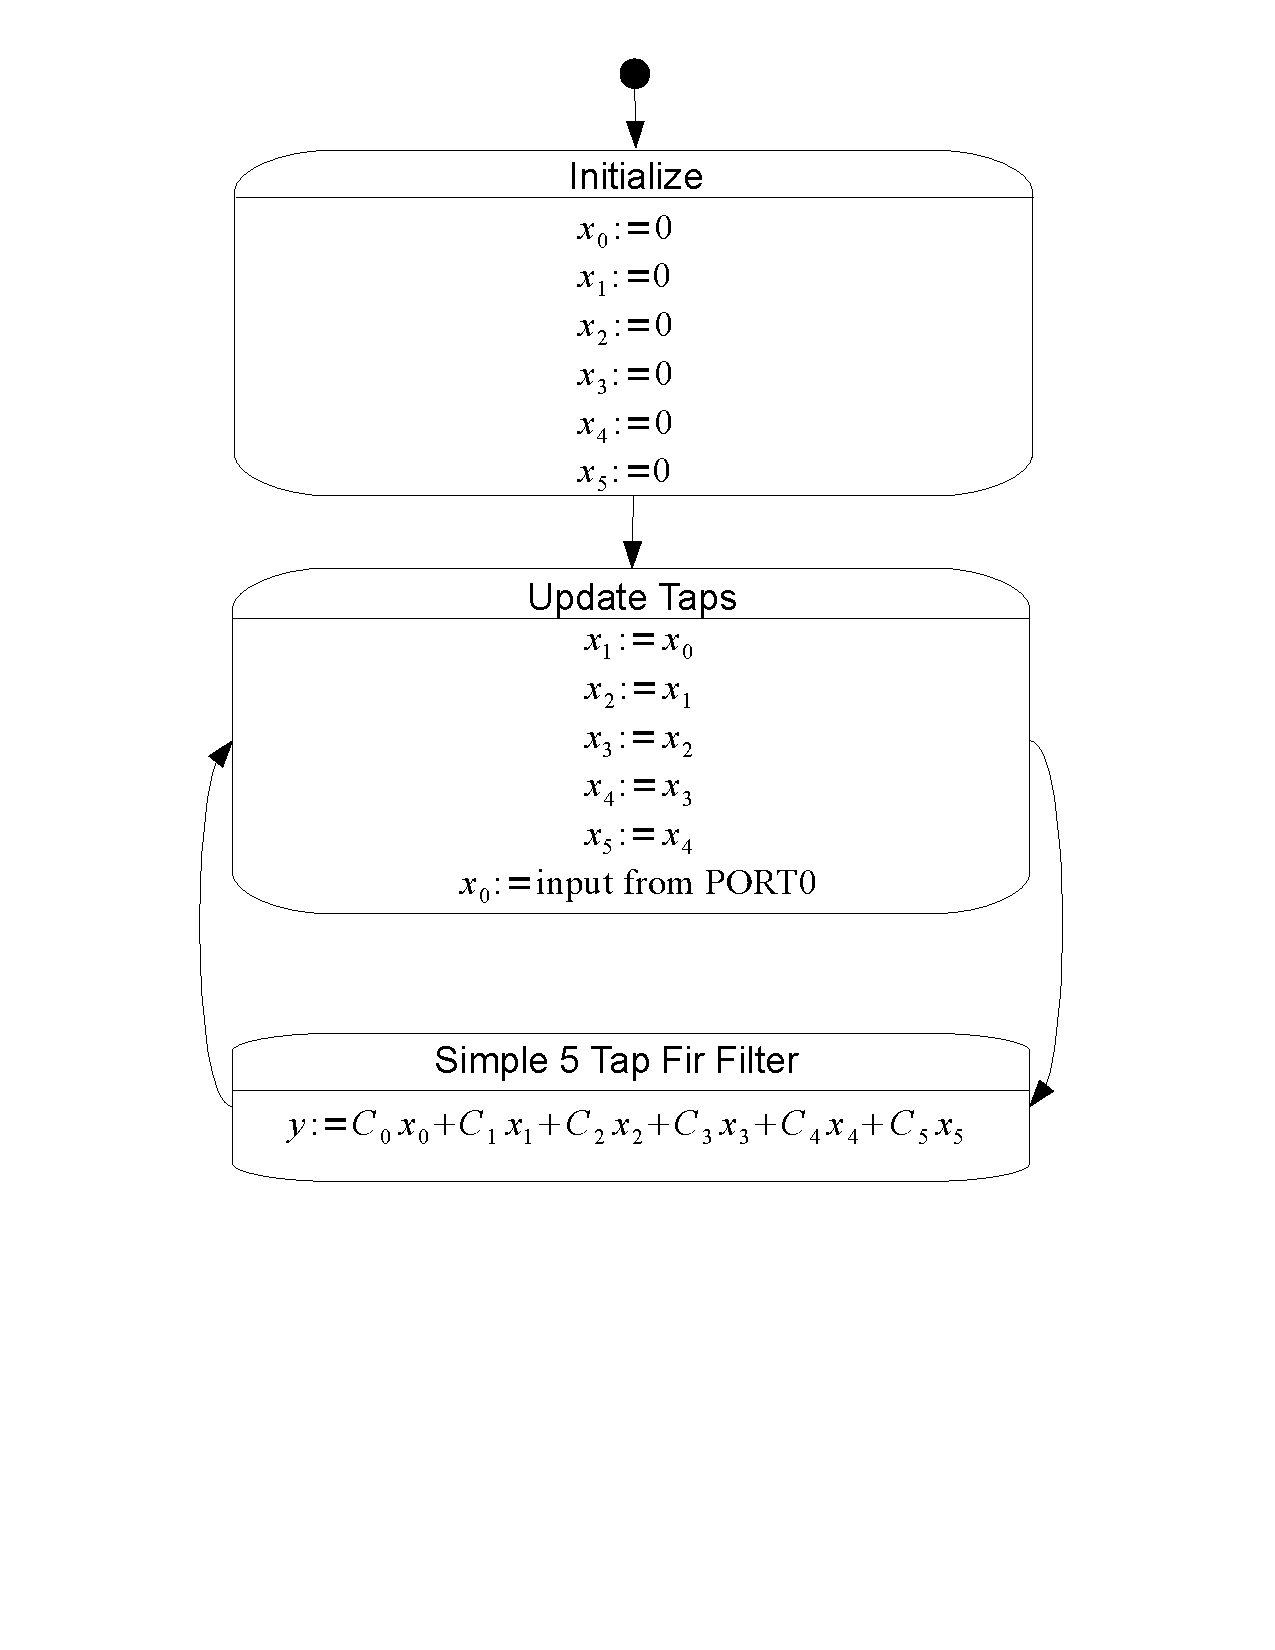
\includegraphics[trim= 10mm 145mm 10mm 10mm, clip, width=\imgmedium]{./images/state_uml2_fir.pdf}
%    \caption{5 Tap Fir Filtering}
%    \label{fig:state_uml2_fir}
%\end{figure}
%
%The advantage of sequential assignments over concurrent assignments can be seen when trying to compute the 5 stage fir filter as seen in figure \ref{fig:state_uml2_fir}. In figure \ref{fig:state_uml2_fir} sequential assignments are very useful for the initial step without it many more modes would be required to do each simple assignment. Thus although this design choice slightly deviates from \emphasize{UML2 State Machine Diagram}\cite{UML2} it was decided the benefits to usability was too great to strictly adhere to the \emphasize{UML2 State Machine Diagram}\cite{UML2} semantics.

\begin{figure}[htp]
    \centering
    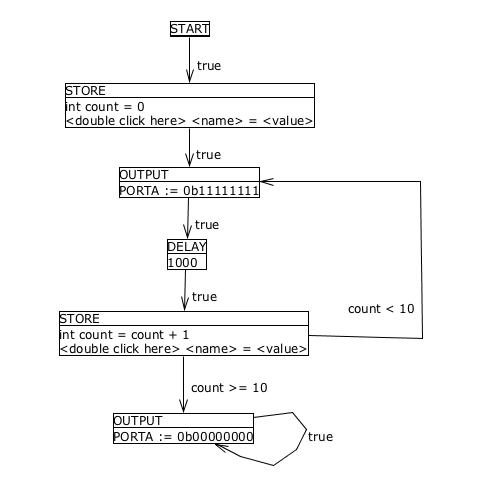
\includegraphics[width=230px]{./images/tool_transition_example.png}
    \caption{PLC Edit Example}
    \label{fig:tool_transition_example}
\end{figure}

\begin{figure}[htp]
    \centering
    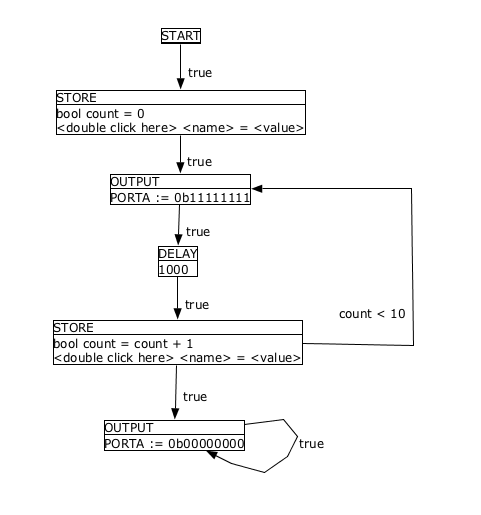
\includegraphics[width=230px]{./images/tool_transition_example_bad.png}
    \caption{PLC Edit Example With Bad Transitions}
    \label{fig:tool_transition_example_bad}
\end{figure}

Transitions in the language must be mutually exclusive. It is invalid to have two transitions that can both be taken at any point. Figure \ref{fig:tool_transition_example} shows an example of this done correctly the two guard conditions ``count $<$ 10'' and ``count $\geq$ 10'' ensure mutual exclusivity. When mutual exclusion is not ensured such as in figure \ref{fig:tool_transition_example_bad} the behaviour of the language is undefined. \plccharts currently does not allow for concurrent execution. Therefore multiple possible edges are ambiguous and the outcome (as in which edge would be taken) is undefined.